\section{系统设计}
\subsection{总体架构模型设计}
\subsubsection{前端架构模型}
\begin{figure}[htb]
    \centering
    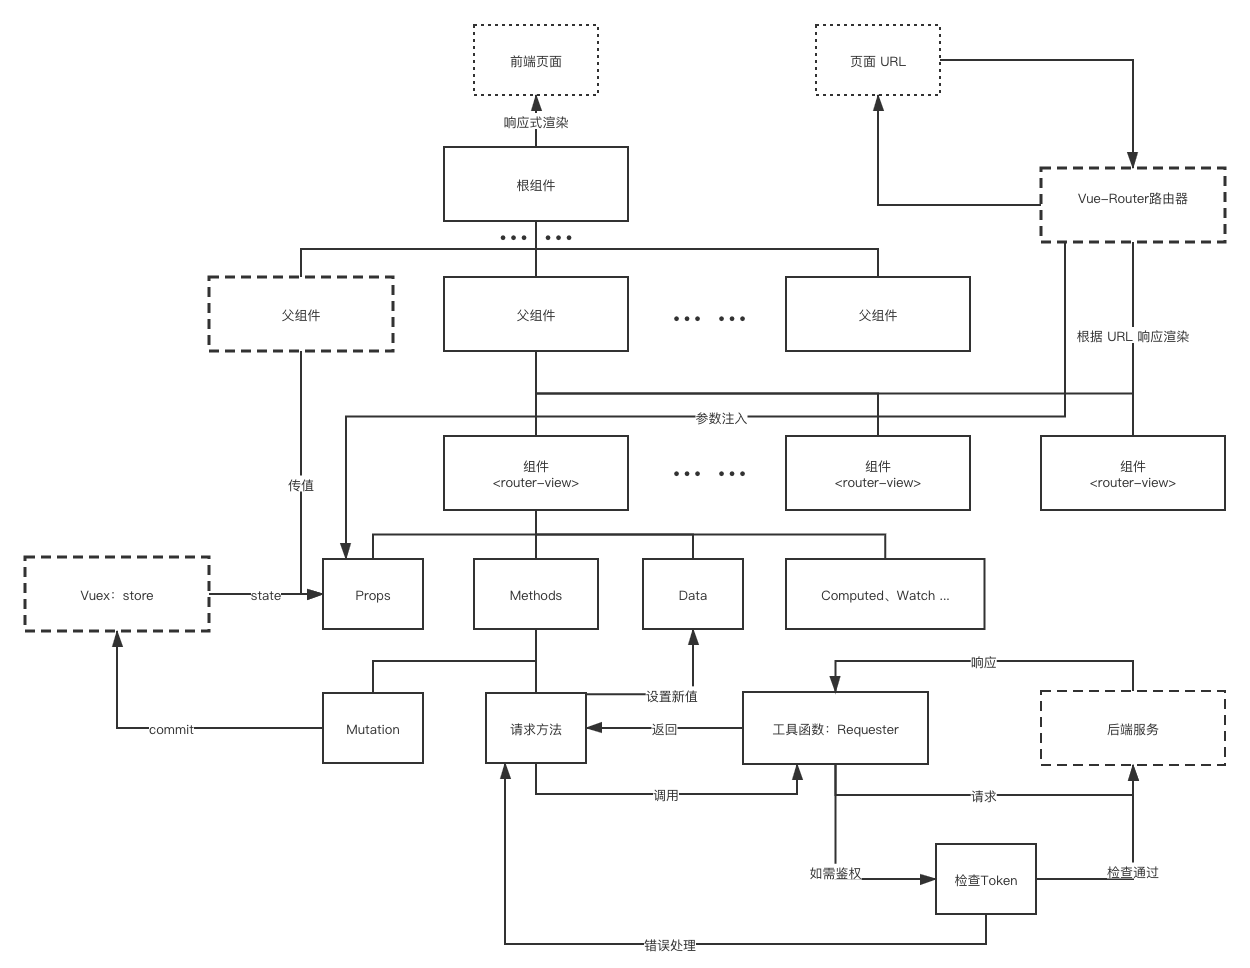
\includegraphics[width=\linewidth]{_images/前端模型.png}
    \caption{前端架构模型}
\end{figure}
Vue 的技术基础是将根节点组件挂载在页面的一个 DOM 元素上,而根节点组件由可由多个组件组成,如此向下细分成子组件。组件系统是 Vue 的另一个重要概念,因为它是一种抽象,允许我们使用小型、独立和通常可复用的组件构建大型应用。\upcite{ref19}

组件的数据来源可以划分为:Props、Data、Computed。父子组件之间的数据通信通过 Props,而 Vue 的设计理念中,数据是自上而下单向流动。

面对需要多组件之间共享公共的数据的场景,需要引入 Vuex 的 store。store 将托管的公有数据 state,通过预先在根节点的注册,注入到需要的组件的 Props 中。如有需要对 store 中的数据进行修改,可以将 store 的 mutation 注入到组件的 Methods 中,通过提交(commit)mutation 实现对 store 中的 state 修改。

组件的 Data 也可能来自于用户的交互产生,又或是向后端服务请求的数据。组件中的请求方法,通过调用工具函数 Requester 向后端服务发起请求,其中如有必要应进行 Token 用户令牌的检查。响应得到的数据将返回给请求方法,进而给组件的 Data 赋予新值。

组件的渲染可能受控于父组件的逻辑,也可能受路由器的控制。在父组件中注册成为 <router-view> 的子组件,就通过 Vue-Router 的路由器,根据页面的 URL 动态响应渲染。其中也可以通过页面的 URL 动态路由匹配,向组件的 Props 注入匹配到的参数。


\subsubsection{后端架构模型}
\begin{figure}[htb]
    \centering
    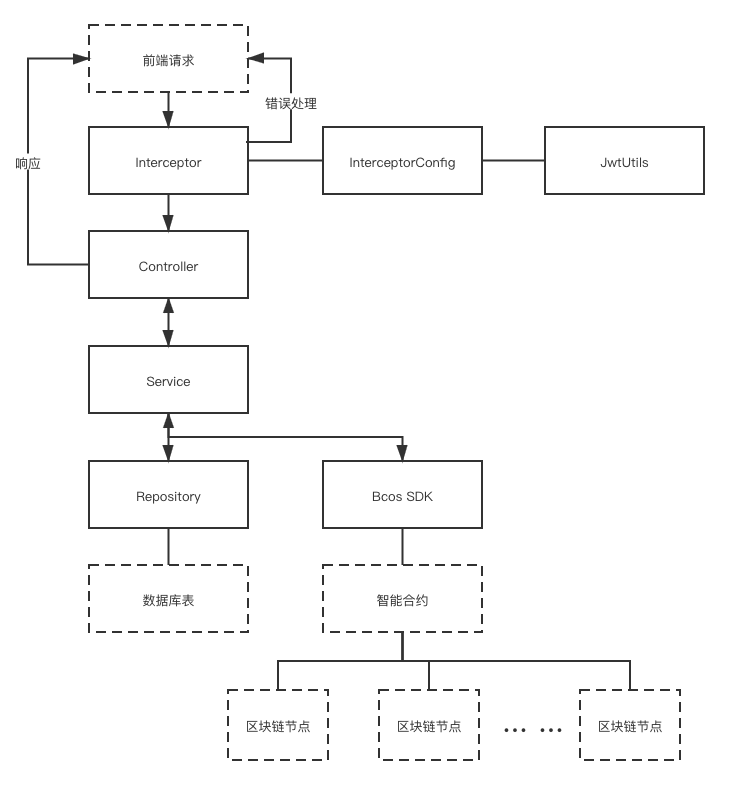
\includegraphics[width=0.85\linewidth]{_images/后端模型.png}
    \caption{后端架构模型}
\end{figure}
前端请求进入后端服务首先会被拦截器 Interceptor 所截获。通过 InterceptorConfig 配置需要拦截的 api 的 url 规则,并加入对应的 Interceptor。项目中的 JWT 鉴权流程便放在拦截器这一层运行。

请求根据具体 api 的 URL,进入不同的 controller,controller 根据业务调用对应的 Service 中的方法。由于使用了 SpringData JPA,数据库中的表与 Repository 对应且关联,因而 Service 中对 DAO 的操作则需要依赖于 Repository。

针对敏感数据需要上链的 Service,通过 Fisco Bcos 提供的 SDK,接入预先编译成 Java 文件的智能合约。而智能合约由通过密钥对的形式连接至区块链节点组成的网络。

\subsection{模块划分}
\begin{figure}[htb]
    \centering
    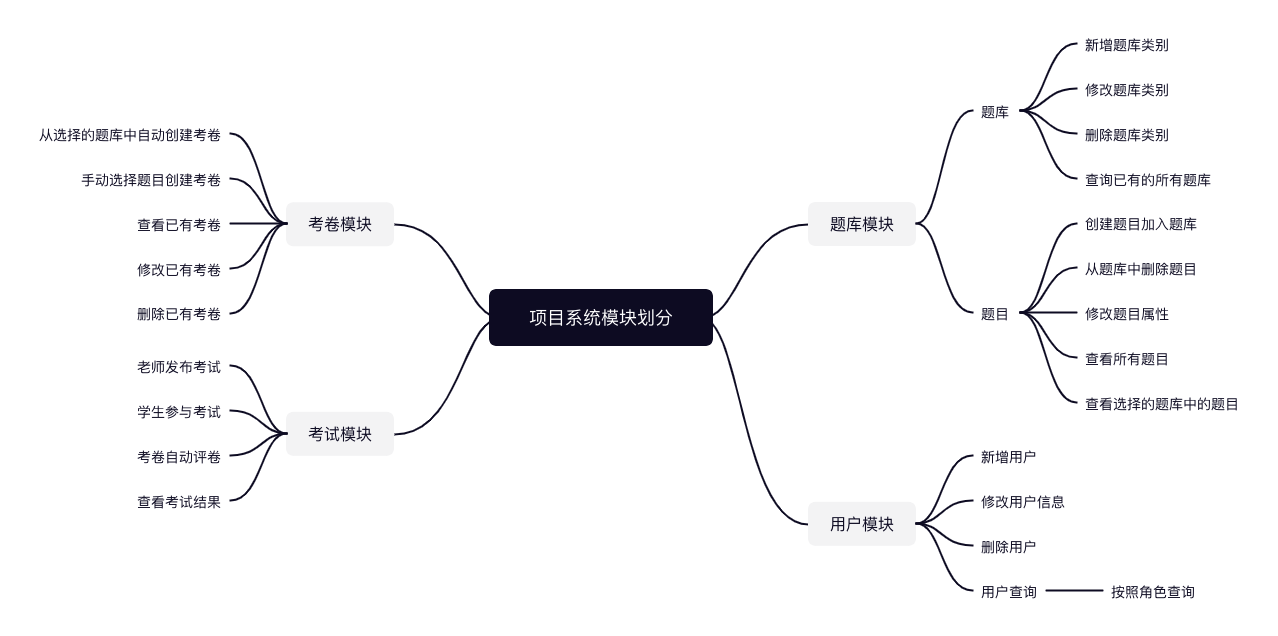
\includegraphics[width=\linewidth]{_images/功能模块划分.png}
    \caption{功能模块划分}
\end{figure}
项目系统根据功能划分成几个功能模块:题库模块、用户模块、考卷模块、考试模块。

按照权限分类用户角色,其对应的功能模块为:\upcite{ref4}
\begin{itemize}
    \item 学生:考试模块
    \item 老师:题库模块、考试模块、考卷模块
    \item 管理员:题库模块、考试模块、考卷模块、用户模块
\end{itemize}

\subsection{Http 请求响应}
\subsubsection{前端请求}
\noindent\textit{front/Requester.js/post函数}
\begin{lstlisting}
function post(url, params = {}, needToken = true) {
    const {token} = TokenManager.getToken()
    ... ...
    Logger.log('request', {url, params})
    return axios({
        method: 'post',
        url: url,
        responseType: 'json',
        data: params,
        headers
    }).then(response => {
        const {data, status, statusText} = response
        Logger.log('response', data)
        return data
    }).catch(reason => {
        const {status, statusText} = reason.response
        Logger.error('response', status, statusText, reason.response)
        throw reason.response
    })
}
\end{lstlisting}
前端的请求发起主要依赖于基于 xhr 实现的第三方库 axios。axios 由于请求的异步延时特性,所以使用了 Promise 进行了封装。

前端对后端的请求过程中,请求的 url 前缀部分都是相同的。此外,对于常用的 POST、GET 方法,请求头部分也有相似的部分,例如,POST 请求统一使用「application/json」的 content-type,并将具体的请求数据 json 序列化后,通过 axios 的 data 字段写入请求体中。因而,可以对 axios 再做一层定制,封装成项目的工具函数集合 Requester 中 post、get。

在业务流程中,使用 Requester,仅仅需要根据请求的方法,调用对应的 post、get,传入对应的 api 的 url、请求参数 params,和是否需要 token 验证的标志位 needToken。而无需关心其中具体的请求配置,以及响应的错误处理。获取响应以后再通过一层 Promise 解构其中真正需要的响应数据,使得在业务层面对于请求-响应中的细节是透明无感知的,从实际意义上的减轻了业务开发过程中的心智负担。并可以在工具函数 Requester 中加入日志输出,以便在线上部署后,通过日志迅速定位错误信息。

\subsubsection{后端响应}
\noindent\textit{back/ResultVO.java}
\begin{lstlisting}[language=Java] 
@Data
@JsonInclude(JsonInclude.Include.NON_NULL) 
public class ResultVO<T> {

    public ResultVO(Integer code, String msg, T data) {
        this.code = code;
        this.msg = msg;
        this.data = data;
    }

    public ResultVO() {}

    private Integer code;

    private String msg = "";

    private T data;
}
\end{lstlisting}

\noindent\textit{back/ExamController.java/getExamRecordList函数}
\begin{lstlisting}[language=Java]
@GetMapping("/record/list")
@ApiOperation("获取当前用户的考试记录")
ResultVO<List<ExamRecordVo>> getExamRecordList(HttpServletRequest request) {
    ResultVO<List<ExamRecordVo>> resultVO;
    try {
        // 拦截器里设置上的用户id
        String userId = (String) request.getAttribute("user_id");
        // 下面根据用户账号拿到他(她所有的考试信息),注意要用VO封装下
        List<ExamRecordVo> examRecordVoList = examService.getExamRecordList(userId);
        resultVO = new ResultVO<>(0, "获取考试记录成功", examRecordVoList);
    } catch (Exception e) {
        e.printStackTrace();
        resultVO = new ResultVO<>(-1, "获取考试记录失败", null);
    }
    return resultVO;
}
\end{lstlisting}

后端的响应部分更多的是借助 SpringBoot 中 \lstinline!starter-web! 启动器所提供的相关框架能力。针对响应体的自定义封装,主要是使用了 ResultVO 这一值对象(Value Object)。其中定义了针对业务而言的状态码 code,即业务操作成功为 0,业务操作失败则为非 0。随之附带 msg 作为扩展的信息说明字段。并且 \lstinline!ResultVO! 通过泛型 \lstinline!<T>! 注入具体响应时的数据类型。例如,\lstinline!getExamRecordList! 函数中展示的,针对当前业务操作需要的是 \lstinline!List<ExamRecordVo>! 的数据类型,因而,在 try-catch 前初始化的响应结果 \lstinline!resultVO! 就是 \lstinline!ResultVO<List<ExamRecordVo>>!。

\subsection{鉴权设计}
针对前后端分离的项目结构,鉴权设计主要是借助 JWT(JavaScript Web Token)这一通用的解决方案完成。
\subsubsection{前端鉴权}
\noindent\textit{front/TokenManager.js}
\begin{lstlisting}[language=JavaScript]
// 设置 Token
function setToken({token, userInfo}, remember = false) {
    if (remember) {
        // 写入 localStorage
        localStorage.setItem(...)
    }
    // 在 store 中设置值
    store.commit(...)
    ... ...
}

// 获取 Token
function getToken() {
    let token, userInfo
    if (store.getters.getToken) {
        token = store.getters.getToken
    }
    if (store.state.auth.userInfo) {
        userInfo = store.state.auth.userInfo
    }
    if (!token && localStorage.getItem(tokenKey)) {
        token = localStorage.getItem(tokenKey)
        userInfo = JSON.parse(localStorage.getItem(userInfoKey))
        // 在 store 中设置值
        store.commit(...)
        ... ...
    }
    return {
        token, userInfo
    }
}

// 移除 Token
function removeToken() {
    ... ...
}
\end{lstlisting}
前端部分对于 Token,以及可以与 Token 视作相关联的敏感用户信息 UserInfo,都使用相同的存储管理思路。

针对登录时勾选了“记住登录状态”的情况,将 Token 以及 UserInfo 写入浏览器提供的 localStorage 中。localStorage 是浏览器提供的一种缓存能力,写入 localStorage 中的键值对,可以持久化存储,使得在浏览器退出后也不会丢失。

针对普通的登录情况,则将这些重要数据写入 Vuex 提供的 store 中,方便各组件获取和修改。

如果重新打开浏览器进入页面,且有勾选“记住登录状态”的情况,store 中已有的 Token 是因为进程退出而丢失的,然而 localStorage 中可能还存有未过期的 Token。因而,在 TokenManager 的 getToken 函数中,需要首先检查 store 中是否有保存 Token,如果没有则再在 localStorage 中读取。如果 localStorage 中读取成功,则说明用户是有勾选了“记住登录状态”,则需要将 Token 作为函数返回值之前,将读取到的 Token 存储到 store 中。

Token 存储的情况有多种,但是移除的时候无需关心是否存在,只需要一并清空 store 和 localStorage 中可能存在的键值对即可。

\noindent\textit{front/Requester.js/post函数}
\begin{lstlisting}[language=JavaScript]
function post(url, params = {}, needToken = true) {
    const {token} = TokenManager.getToken()
    if (needToken && !token) {
        Logger.error('not found token')
        return Promise.reject({
            code: 1401,  // 浏览器的401
            msg: 'not found token'
        })
    }
    const headers = {}
    if (needToken) {
        headers['Access-Token'] = `bearer ${token}`
    }
    ... ...
}
\end{lstlisting}

在 Requester 工具函数中,请求如果设置了 needToken 的标志位,则使用 TokenManager 的 getToken 函数中读取可能存在的 Token。如此设计,在请求的代码编写中,将两个模块解耦,仅仅通过函数调用相互关联,符合“高内聚,低耦合”的设计原则。

如果需要 Token 而 getToken 无法返回有效 Token 时,则需要进行错误的处理。遵照 axios 的 Promise 风格 api,错误处理也使用相似的 Promise.reject。其中自定义状态码设置为“1401”,意图借 HTTP 状态码的 401 相同的含义,再前加上 1,以示区别。

getToken 成功返回 Token 后,则通过请求头中的 Access-Token 字段,在请求中携带上 Token。

\noindent\textit{front/Requester.js/handleRequestError函数}
\begin{lstlisting}[language=JavaScript]
function handleRequestError(error) {
    if (
        (
            error && typeof (error) === 'object' &&
            error.code > 1400 && error.code < 1500
        ) || error.status === 401
    ) {
        TokenManager.removeToken()
    }
    Logger.error(error)
}
\end{lstlisting}

对于如上的需要 Token,而又没有 Token 的特殊处理情况,则通过 handleRequestError 对于前面定义的特殊状态码“1401”做处理动作,在当前的项目中,仅仅只是调用了 removeToken。但是,将这个针对 Token 的错误处理环节的独立抽离,也是意图方便以后可能会加入的新的错误处理逻辑,使得项目代码留存有一定的扩展空间。

\subsubsection{后端鉴权}
\noindent\textit{back/LoginInterceptor.java/preHandle函数}
\begin{lstlisting}[language=Java]
@Override
public boolean preHandle(... ...) throws Exception {
    ... ...
    // 注意要和前端适配Access-Token属性,前端会在登陆后的每个接口请求头加Access-Token属性
    String token = request.getHeader("Access-Token");
    ... ...
    if (token != null) {
        // 请求中是携带参数的
        Claims claims = JwtUtils.checkJWT(token);
        if (claims == null) {
            // 返回null说明用户篡改了token,导致校验失败
            sendJsonMessage(response, JsonData.buildError("token无效,请重新登录"));
            return false;
        }
        ... ...
        return true;
    }
    ... ...
    return false;
}
\end{lstlisting}
后端的鉴权与前端部分相对应,而后端的请求鉴权主要是通过 SpringBoot 提供的拦截器 \lstinline!Interceptor! 框架能力完成。拦截器通过配置对应的拦截规则,调用对应的拦截器,可以实现需要鉴权的请求在进入实际的业务代码 \lstinline!Controller! 层之前,在拦截器中进行鉴权。将其这部分鉴权逻辑单独通过拦截器实现,目的是为了同业务代码独立开,互相不影响。如此的设计,也是遵从了“低耦合”的原则思想。
\begin{lstlisting}[language=Java]
public class JwtUtils {
    // 构建 token 的主题
    private static final String SUBJECT = ... ...;
    // 过期时间为1天
    private static final long EXPIRE = 1000 * 60 * 60 * 24;

    private static final String APP_SECRET = ... ...;

    public static String genJsonWebToken(User user) {
        ... ...
        return Jwts.builder().setSubject(SUBJECT)
                // 下面3行设置 token 中间字段,携带用户的信息
                ... ...
                // 设置过期时间
                ... ...
                // 生成的结果字符串太长,这里压缩下
                .compact();
    }

    /* 校验 token */
    public static Claims checkJWT(String token) {
        ... ...
    }
}
\end{lstlisting}

将 jsonwebtoken 提供的 api 能力针对项目的业务情况再进行一次封装,成为 \lstinline!JwtUtils! 工具。对外仅提供了对 Token 的创建、校验能力。

\subsection{数据库结构设计}
\subsubsection{数据库概念设计}
\begin{figure}[htb]
    \centering
    \includegraphics[width=\linewidth]{_images/ER图.png}
    \caption{数据库ER图}
\end{figure}

\subsubsection{数据库逻辑设计}
\begin{lstlisting}
users(
    userId, username, password, roleId, avatar,
    nickname, description, createTime, updateTime
)
exam_paper( examPaperId, name, avatar, questionIds, score, creatorId )
exam( id, name, avatar, startDate, endDate, timeLimit, creatorId )
question_bank( id, name, questionIds, creatorId, ... )
question( id, name, description, optionIds, ... )
\end{lstlisting}
\subsubsection{数据表字段说明}
\paragraph{users}
\begin{itemize}
    \item userId 为表的主键,用于唯一标识一个用户;
    \item username 为用户的登录时所用名称,与 userId 一样不可重复;
    \item avatar 存储用户头像;
    \item roleId 存储用户对应的权限角色的枚举值;
    \item nickname 存放用户的昵称,可重复,仅用于展示;
    \item password 为用户登录时所使用的密码;
\end{itemize}
\paragraph{exam\_paper}
\begin{itemize}
    \item examPaperId 为表的主键,用于唯一标识一张考卷;
    \item name 存放考卷的名称;
    \item avatar 存放考卷的封面,可为空;
    \item questionIds 存放考卷拥有的题目的 id 集合;
    \item score 表示考卷的总分值;
    \item creatorId 存放创建考卷的用户的 id(外键);
\end{itemize}
\paragraph{exam}
\begin{itemize}
    \item id 为表的主键,用于唯一标识一场考试;
    \item name 表示考试的名称;
    \item startDate、endDate 表示考试的有效日期范围;
    \item timeLimit 表示考试的答题时间;
    \item creatorId 存放创建考试的用户的 id(外键);
\end{itemize}